\documentclass[a4paper, 12pt, twoside]{report}
\usepackage[T1]{fontenc}
\usepackage[utf8]{inputenc}
\usepackage[italian]{babel}
\usepackage{graphicx}
\usepackage{wrapfig2}
\usepackage{amsmath}
\usepackage{cases}
\usepackage{subcaption}
\usepackage{hyperref}
\hypersetup{
	colorlinks=true,
	linkcolor=blue,    
	urlcolor=blue,
	pdfpagemode=FullScreen,
}
\urlstyle{same}
\raggedbottom

\begin{document}
	\setcounterpageref{secnumdepth}{0}
	\title{Relazione esperienza di laboratorio \\ Corso di elettrotecnica \\ A.A 2021-2022}
	\author{Andrea Marchegiani mat. 810513}
	\date{10/05/2022}
	\maketitle
		
	Nell'esperienza svolta è stato possibile applicare e visualizzare la legge di carica e di scarica di un condensatore di capacità C in serie ad un resistore di resistenza R. {}
	Si visualizzeranno infine i transitori di carica e di scarica attraverso un oscilloscopio dimostrando come i valori e gli andamenti attesi combaceranno con quelli reali. {} 	
	
	
\begin{wrapfigure}{l}{0.25\textwidth}
		\includegraphics[width=1\linewidth]{"Carica&Scarica/Scarica RC"}
		\label{fig:RC}		
\end{wrapfigure}

\paragraph {Scarica di un condensatore} \mbox{} \newline
Il condensatore è un bipolo conservativo caratterizzato dal seguente legame tensione - corrente:
\begin{equation}
	\label{1:1}
 i\left(t\right) = dC\left(t\right) {\frac{v\left(t\right)}{dt}}
\end{equation}
Il parametro C è detto Capacità e la sua unità di misura è il Farad [F].
Nel caso di invarianza temporale delle caratteristiche fisiche e geometriche, il legame costitutivo di un condensatore diviene: 
\begin{equation}
	\label{1:2}
i\left(t\right)=C\frac{dv\left(t\right)}{dt}
\end{equation}
 Un transitorio può generalmente immaginarsi dovuto all’apertura o alla chiusura istantanee di interruttori che escludano o inseriscano uno o più componenti circuitali.{}
 
Nel transitorio di scarica ivi analizzato si suppongono sia il condensatore inizialmente carico ad una generica tensione $v_{c0}$, sia che nell’istante $t=0$ l’interruttore si chiuda. In questo modo l'energia immagazzinata nel condensatore inizierà a fluire nel circuito sotto forma di corrente, fino a quando la resistenza non l'avrà totalmente dissipata.{}

Si evince pertanto da (\ref{1:1}) e (\ref{1:2}) come la corrente in un condensatore sia in relazione differenziale con la tensione: quest’ultima sarà una variabile CONTINUA nel dominio temporale. 

La POTENZA assorbita da un condensatore è, dalla definizione:
\[
p\left(t\right)=v\left(t\right)i\left(t\right)=v\left(t\right)C\frac{dv\left(t\right)}{dt}
\]

L’energia assorbita dal condensatore nel generico intervallo di tempo $(0,t)$ è quindi:
\begin{equation}
	\begin{split}
w_c\left(0,t\right)=\int_{0}^{t}p\left(t\right)dt=\int_{0}^{t}v\left(t\right)i\left(t\right)dt=\\
=\int_{0}^{t}{v\left(t\right)C\frac{dv\left(t\right)}{dt}dt}= \\
\frac{1}{2}C\int_{0}^{t}{\frac{dv^2\left(t\right)}{dt}dt}= 
\frac{1}{2}C\left[v^2\left(t\right)-v^2\left(0\right)\right]
\end{split}
\end{equation}

L’energia assorbita nell’intervallo considerato dipenderà così esclusivamente dal valore che la tensione sul condensatore assumerà nell’instante iniziale 0 e nell’istante finale t e non dalla sua particolare evoluzione temporale.

La tensione sul condensatore prende così la forma di una FUNZIONE DI STATO sia perché legata all’energia immagazzinata, sia perché la variazione tra gli istanti temporali considerati - stati del sistema - dipende solamente dal valore delle coordinate di questi ultimi. Si ricorda inoltre che una funzione di stato ammette sempre un differenziale esatto. {

Infine, poiché si è dimostrata la tensione sul condensatore essere una funzione di stato, è chiaro come questa NON potrà variare istantaneamente valore in modo discontinuo, di conseguenza, nel circuito in analisi il valore della tensione non potrà che rimanere lo stesso sia prima che nell’istante immediatamente successivo alla chiusura dell’interruttore:
 
 \[
 	\begin{cases}
v_C (0^-)=v_{C0} \\
i(0^- )=0A
 	\end{cases}
\Rightarrow v_C (0^-)=v_C (0^+)=v_{C0}
 \]

Dalla legge di Ohm si ottiene la corrente circolante nella maglia:
\[
i\left(t=0^+\right)=\frac{v_{c0}}{R}
\]
Esaurita la fase transitoria il condensatore si sarà scaricato e flusso di corrente si arresterà:
\[
i_C\left(t=\infty\right)=0A;v_C\left(t=\infty\right)=Ri_C\left(t\right)=0
\]

Alla chiusura dell’interruttore si evidenzieranno le seguenti relazioni:
\[
i\left(t\right)=-i_C=-\frac{Cdv_C}{dt};i\left(t\right)=\frac{v_R}{R};v_R=v_C
\]

Di conseguenza è possibile scrivere l’equazione risolutiva:
\begin{equation}
-\frac{Cdv_C}{dt}=\frac{v_C}{R}
\end{equation}

Si tratta di un’equazione differenziale del primo ordine a coefficienti constanti, lineare ed omogenea la cui soluzione è quindi:
\[
v_C\left(t\right)=A\ e^{-\frac{t-t_0}{\tau}}
\]
Se $t_0=0$
\begin{equation}
v_C\left(t\right)=A\ e^{-\frac{t}{\tau}}
\end{equation}


Per trovare il valore di $\tau$ è possibile sostituire nell’equazione risolutiva la soluzione generica:
\[
	\begin{split}
-C\frac{d\left(A\ e^{-\frac{t}{\tau}}\right)}{dt}=\frac{A\ e^{-\frac{t}{\tau}}}{R}\\
C\frac{1}{\tau}Ae^{-\frac{t}{\tau}}=\frac{Ae^{-\frac{t}{\tau}}}{R}\\
\tau=RC
\end{split}
\]
$\tau$ è detta anche costante di tempo del sistema. Dimensionalmente è un tempo espresso secondi. Essa indica la velocità dell’evoluzione del sistema risultando un parametro di scala della variabile tempo.
Per trovare il valore del coefficiente A si può utilizzare la seguente condizione, per $t=0^+$
\[
v_C\left(0^-\right)=v_C\left(0^+\right)=v_{C0}
A=v_{C0}
\]

Di conseguenza, gli andamenti della tensioni ai capi del condensatore e della corrente nel circuito sono: 
\begin{equation}
	\begin{split}
v_C=v_{C0}e^{-\frac{t}{\tau}}\\
i=\frac{v_{C0}}{R}e^{-\frac{t}{\tau}}
\end{split}
\end{equation}

Dopo un intervallo temporale che va dai $4\tau \div 5\tau$ il transitorio si esaurisce, scende al $2-3\%$ del valore di partenza. 

\begin{figure}[H]
	\centering
	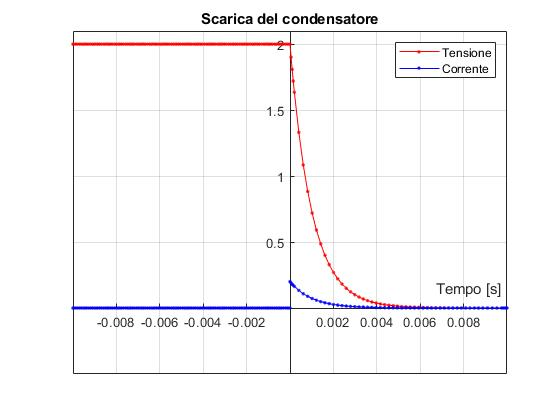
\includegraphics[width=1\linewidth]{Carica&Scarica/plotScaricaRCfig}
	\caption{scarica del circuito RC}
	\label{fig:PLOTRC}
\end{figure}

\begin{wrapfigure}{l}{0.25\textwidth}
	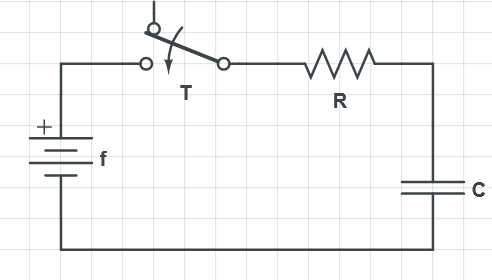
\includegraphics[width=1.0\linewidth]{Carica&Scarica/Carica RC}
\end{wrapfigure}

\paragraph {Transitorio del I ordine: Carica del circuito ERC}	\mbox{} \newline

Si supponga anche in questo caso il condensatore sottoposto ad una tensione $v_{C0}$ per cui:
\[
	\begin{cases}
		v_c (0^-)=v_C0 \\
		i(0^- )=0A
	\end{cases}
\]

Nell’istante $t=0$ l’interruttore si chiude e il condensatore si troverà connesso in serie ad una resistenza e ad un generatore di tensione.

Quella che inizierà a fluire sarà ora una corrente che in questo caso caricherà il condensatore fino al nuovo equilibrio.

Come ampiamente dimostrato la tensione sul condensatore è una funzione di stato, non variando quindi impulsivamente di valore, manterrà lo stesso invariato anche nell’istante immediatamente successivo alla chiusura dell’interruttore:
\[
v_C\left(0^-\right)=v_C\left(0^+\right)=v_{C0}
\]

Cosa accade perciò nelle varie finestre temporali? 

A $t<0$ il circuito è aperto, non scorre corrente nè per mano del condensatore carico, nè per mano del generatore di tensione.

A $t=0$ definiamo il transitorio del circuito.
Tutti i bipoli vengono attraversati dalla stessa corrente I. Attraverso le Leggi di Kirchhoff alle Tensioni si può scrivere:
\[
E=v_R\left(t\right)+v_C\left(t\right)\ 
\]
Per risolvere il circuito è però necessario considerare sia le equazioni caratteristiche del condensatore che del resistore, giungendo a:
\begin{equation} 
E=RC\frac{dv_C}{dt}+v_C
\end{equation}

Si tratta anche questa di un’equazione differenziale del primo ordine a coefficienti costanti, lineare, ma questa volta non omogenea.
Per cui, riordinando i termini e imponendo le condizioni iniziali che prevedono una tensione ai capi del condensatore uguale sia per $0^-$ che per $0^+$, si ha il seguente problema di Cauchy:
\begin{equation}
	\begin{cases}
		\frac{dv_C\left(t\right)}{dt}+\frac{1}{RC}v_C\left(t\right)=\frac{E}{RC} \\
		 v_C\left(0\right)=V_{C0}
	\end{cases}
\end{equation}

Che come soluzione avrà:

\begin{equation}
v_C\left(t\right)=v_C^0\left(t\right)+v_C^p\left(t\right)
\end{equation}

Ove $v_C^0\left(t\right)$ è la soluzione dell’equazione differenziale omogenea associata:
\[
\frac{dv_C\left(t\right)}{dt}+\frac{1}{RC}\ v_C\left(t\right)=0
\]

Che conduce a:
\[
v_C^0\left(t\right)=k\ e^{-\frac{t}{\tau}}
\]

A $t>0$, una volta esaurito il transitorio, la soluzione che governerà il circuito sarà la $v_C^p\left(t\right)$: soluzione particolare. 

In questo caso:
\[
v_C^p\left(t\right)=E
\]

Infine si avrà, unendo le due soluzioni, per $t\ge0$:
\begin{equation}
v_C\left(t\right)=k\ e^{-\frac{t}{\tau}}+E
\end{equation}

Il valore della costante k si determinerà - solo a questo punto - dall’imposizione delle condizioni iniziali del problema di Cauchy:

\[
v_C\left(0\right)=k\ +E=v_{C0}\ ;k=v_{C0}-E
\]

E la soluzione del problema sarà:
\begin{equation}
v_c\left(t\right)=\left(v_{C0}-E\right)e^{-\frac{t}{\tau}}+E
\end{equation}

Nota così la $v_C\left(t\right)$ sarà possibile determinare la corrente che scorre nel circuito applicando la relazione costitutiva del condensatore (\ref{1:2}):

\begin{equation}
i\left(t\right)=C\frac{d}{dt}v_C\left(t\right)=-C\frac{1}{RC}\left(v_{C0}-E\right)e^{-\frac{t}{\tau}}=\frac{E-v_{C0}}{R}e^{-\frac{t}{\tau}}
\end{equation}
La costante $\tau=RC=[s]$ anche in questo caso indica la velocità dell’evoluzione del sistema.

\begin{figure}[H]
	\centering
	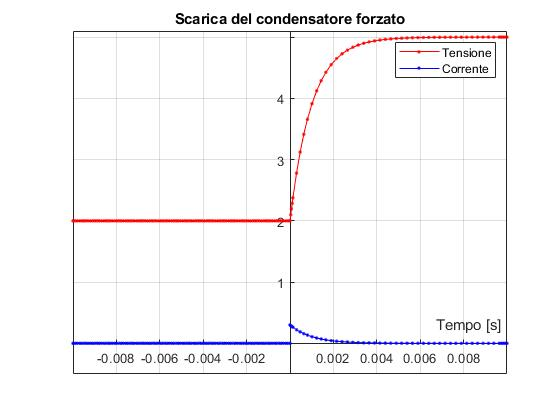
\includegraphics[width=1\linewidth]{Carica&Scarica/plotScaricaERCfig}
	\caption{carica del circuito ERC}
	\label{fig:PLOTERC}
\end{figure}
\newpage
\paragraph {ESPERIENZA}	
\subparagraph{Attrezzatura} \mbox{} \newline

Per l'esecuzione dell'esperienza ci si è avvalsi di:
\begin{itemize}
	\item Una scheda di prototipazione (Breadboard); \newline
	 La breadboard permette di realizzare prototipi di circuiti senza la necessità di eseguire saldature. È una basetta con dei fori nei quali si inseriscono i terminali dei componenti. Il circuito così realizzato può essere facilmente modificato e smontato.
	\item Un resistore dal valore di $R=1.8 ~K\Omega$; 
	\item Un condensatore dal valore di $C_{1}=0.33 ~\mu F$;
	\item Un condensatore dal valore di $C_{2}=2.2 ~\mu F$;
	\item Cavi jumper di collegamento;
	\item Un generatore di segnale; \newline
	Il generatore di funzioni usato in questa esperienza genererà il segnale in tensione che occorrerà fornire al circuito per alimentarlo, in particolare si potrà modificare il segnale di alimentazione. \newline
	Scegliendo un'onda quadra, questa si comporterà periodicamente come se fosse un interruttore, accendendosi (carica) e spegnendosi (scarica). \newline 
	È il generatore di funzioni che si dovrà considerare quando sarà necessario un cambio delle proprietà dell'onda generata (frequenza, ampiezza, \dots ).
	\item Un oscilloscopio. \newline
	Posto a valle del circuito è lo strumento che permetterà la visualizzazione del segnale. Dotato di uno schermo configurabile e di diversi pin di ingresso per il segnale, sarà utilizzato in modo da visualizzare sia il segnale generato (in giallo), che quello misurato sul condensatore (in blu).
\end{itemize}

\begin{figure} [H]
	\centering
	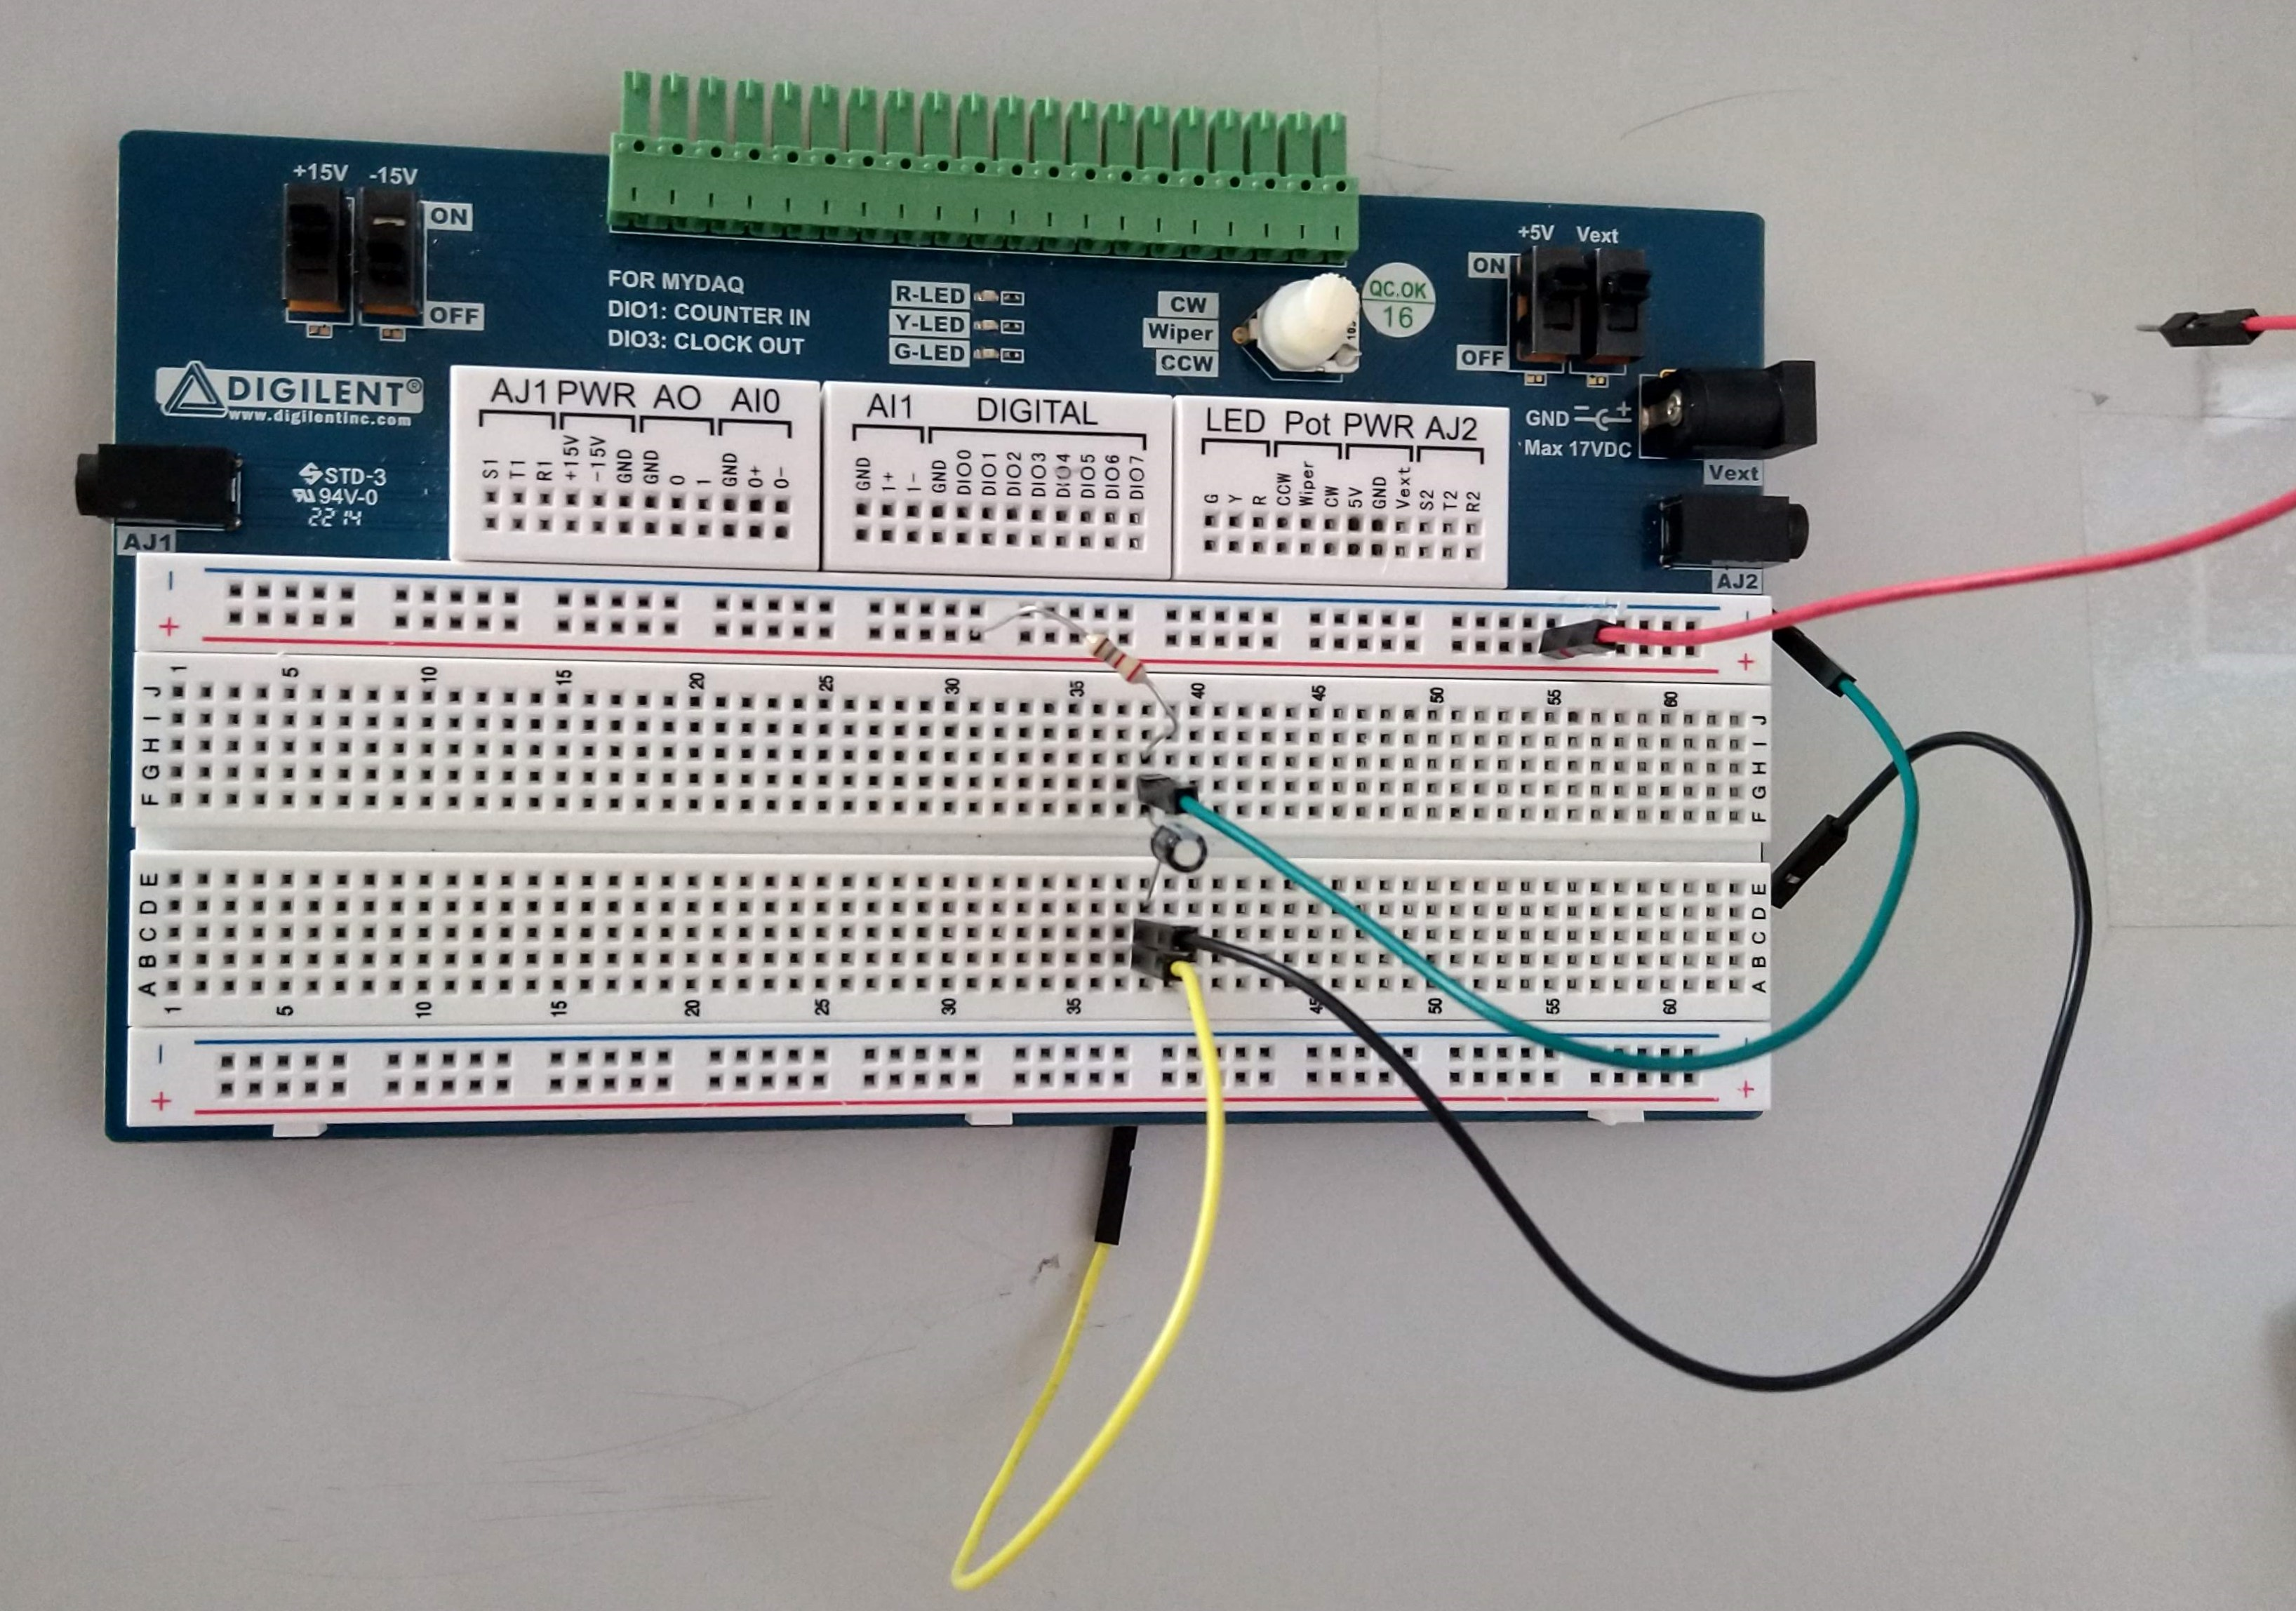
\includegraphics[width=1\linewidth]{Esperienza/Breadboard}
	\caption{Costruzione del circuito sulla Breadboard}
	\label{fig:BB}
\end{figure}



 \subparagraph{Caso 1: Carica completa} \mbox{} \newline
 
 Si visualizzerà il caso in cui, durante il periodo di generazione del segnale, il condensatore riuscirà dapprima a caricarsi completamente, e in seguito a scaricarsi del tutto. 
 
 L'onda quadra agirà come un interruttore: durante la sua accensione il condensatore accumulerà carica, mentre non appena si spegnerà questa verrà rilasciata tendendo a riequilibrare la quantità di carica presente nel circuito, che una volta arrivata alla resistenza si dissiperà. 
 
 In questo caso ci si servirà di un condensatore $C_{1}=0.33 ~\mu F$ e di un'onda quadra a $f_{1}=240 ~Hz$.
 Il tempo caratteristico è:
 \[
 \tau_{Caso1}=RC_{1}=5.94\cdot10^{-4}s=0.594ms
 \]
Adatto a completare un transitorio di carica e di scarica.

Quello che infine si visualizza all'interno di un periodo del segnale sorgente sono transitori completi della durata di un tempo caratteristico: esponenziali intatti di carica e scarica.

\begin{figure}[H]
	\begin{subfigure}{1\textwidth}
		\centering
		% include first image
		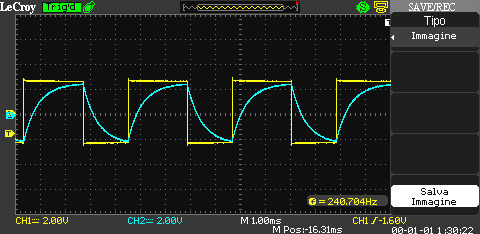
\includegraphics[width=1\linewidth]{Esperienza/ImmaginiOscilloscopio/Caso1}  
		\caption{Immagine dall'oscilloscopio caso1}
		\label{fig:sub1}
	\end{subfigure}
	\begin{subfigure}{1\textwidth}
		\centering
		% include second image
		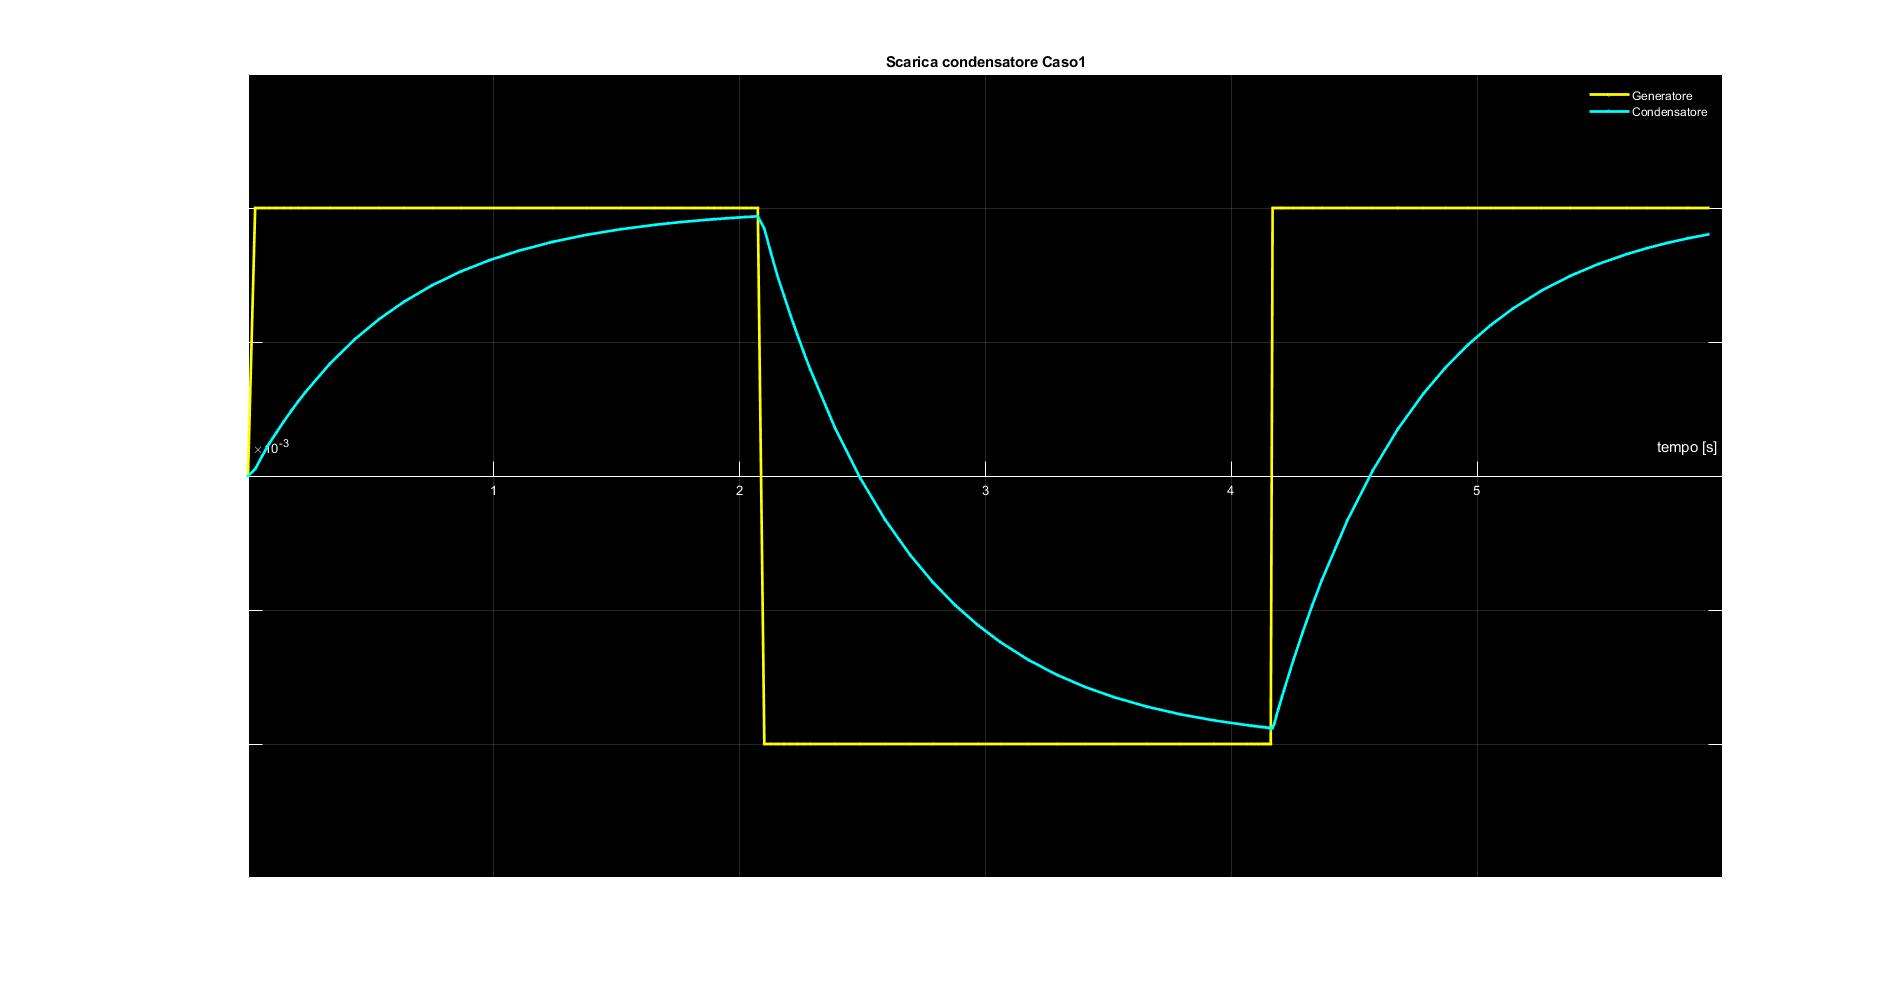
\includegraphics[width=1\linewidth]{Esperienza/MLcaso1}
		\caption{Plot codice MatLab caso1}
		\label{fig:sub2}
	\end{subfigure}
\end{figure}
 

 
   Nei prossimi due casi si visualizzeranno esempi di carica incompleta ottenuti sia agendo sul segnale sorgente, quindi mantenendo il circuito intatto, sia sostituendo il bipolo condensatore.
 
 \subparagraph{Caso 2: Carica incompleta, frequenza} \mbox{} \newline
 
 La carica incompleta si avrà perciò nel momento in cui, durante il periodo di generazione del segnale, il condensatore non riuscirà caricarsi completamente dando luogo ad una scarica incompleta.
 Anche in questo secondo caso ci si avvarrà del condensatore da $C_{1}=0.33 ~\mu F$ ma di un'onda quadra a $f_{2}=750 ~Hz$. 
 Si dimostrerà graficamente in questo caso che anche solo aumentare la frequenza del generatore non darà la possibilità al condensatore di caricarsi completamente.
   
 Il tempo caratteristico rimane lo stesso del primo caso:
 \[
 \tau_{Caso2}=\tau_{Caso1}=RC_{1}=5.94\cdot10^{-4}s =0.594ms
 \]
Questa volta però non è più adatto a completare un transitorio di carica e di scarica a causa della maggior frequenza del segnale sorgente. 

Quelli perciò che si visualizzeranno saranno nientemeno che transitori di carica e scarica incompleti, interrotti. 
   
  \begin{figure}[H]
  	\begin{subfigure}{1\textwidth}
  		\centering
  		% include first image
  		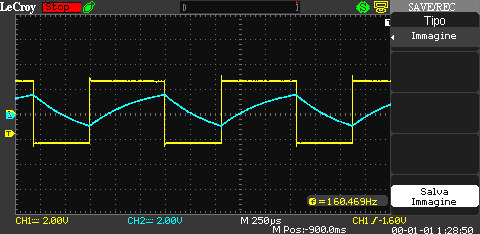
\includegraphics[width=1\linewidth]{Esperienza/ImmaginiOscilloscopio/Caso2}  
  		\caption{Immagine dall'oscilloscopio caso2}
  		\label{fig:sub3}
  	\end{subfigure}
  	\begin{subfigure}{1\textwidth}
  		\centering
  		% include second image
  		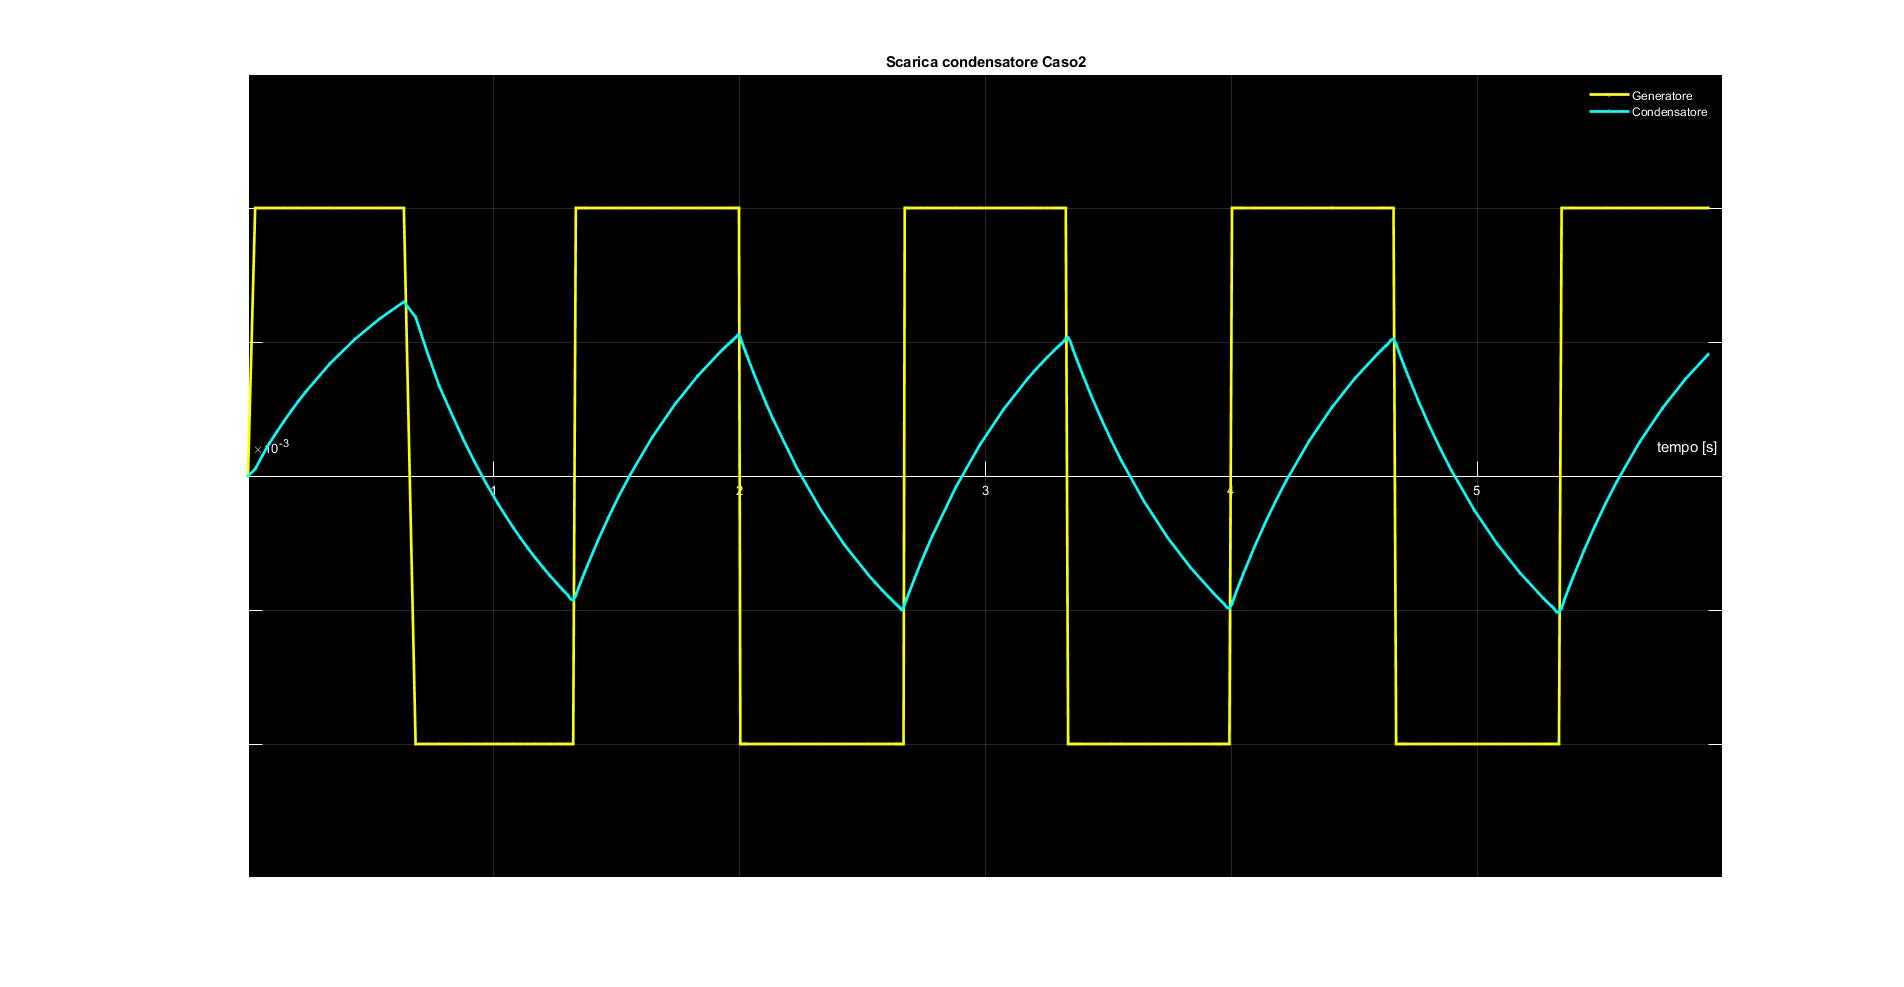
\includegraphics[width=1\linewidth]{Esperienza/MLcaso2}
  		\caption{Plot codice MatLab caso2}
  		\label{fig:sub4}
  	\end{subfigure}
  \end{figure}
   
   \subparagraph{Caso 3: Carica incompleta, capacità} \mbox{} \newline
    
 In quest'ultimo caso si userà il condensatore da $C_{2}=2.2 ~\mu F$ e un'onda quadra di frequenza uguale a quella del caso iniziale $f_{1}=240 ~Hz$.
 Si dimostrerà graficamente che anche solo aumentando la capacità del condensatore in serie al circuito, questo non riuscirà a caricarsi nel periodo del segnale di generazione e darà luogo ad una carica incompleta.

Il tempo caratteristico è dunque:
\[
\tau_{Caso3}=RC_{2}=0.0040s=4ms
\]
Anche in questo caso, ma questa volta a causa di una capacità maggiore, il tempo caratteristico, molto più grande di $\tau_{Caso1}$ non è adatto a completare i transitori di carica e di scarica.

Quelli che si visualizzeranno all'interno di un periodo del segnale sorgente saranno anche qui transitori interrotti, incompleti. 

\begin{figure}[H]
	\begin{subfigure}{1\textwidth}
		\centering
		% include first image
		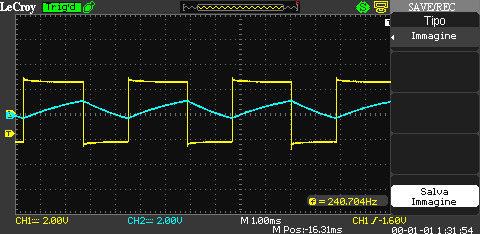
\includegraphics[width=1\linewidth]{Esperienza/ImmaginiOscilloscopio/Caso3}  
		\caption{Immagine dall'oscilloscopio caso3}
		\label{fig:sub5}
	\end{subfigure}
	\begin{subfigure}{1\textwidth}
		\centering
		% include second image
		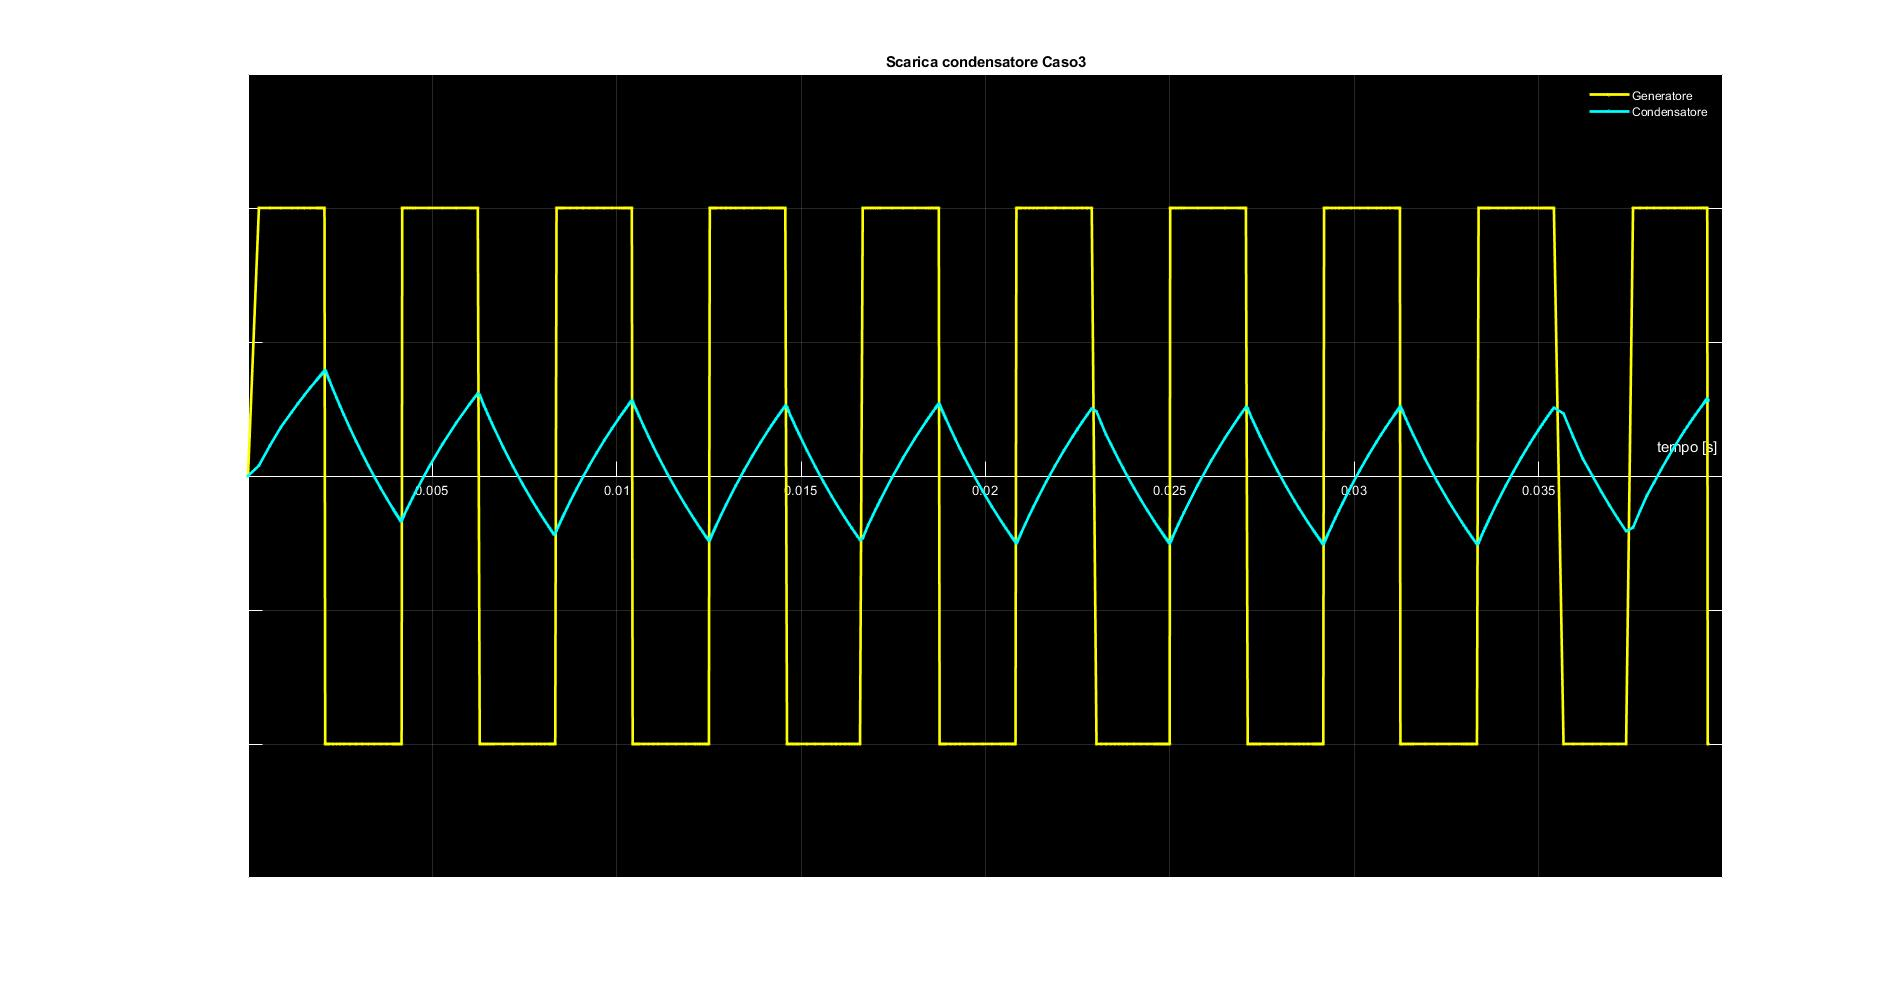
\includegraphics[width=1\linewidth]{Esperienza/MLcaso3}
		\caption{Plot codice MatLab caso3}
		\label{fig:sub6}
	\end{subfigure}
\end{figure}
\begin{tiny}
Si lascia infine una semplice simulazione su Thinkercad del circuito RC appena studiato. \newline
Thinkercad è un software gratuito di disegno 3D, sviluppato dalla Autodesk, che permette anche la costruzione e la simulazione di circuiti elettrici attraverso una BreadBoard virtuale. \newline

\bfseries{NB:}
Non è certamente una simulazione che si prefigge l'essere quanto più completa possibile, ma mi ha dato modo di approfondire l'uso della BreadBoard e i collegamenti da effettuare su di essa prima di effettuarli nella giornata di laboratorio.

\centering
\href{https://www.tinkercad.com/things/k6fuBPthn0e?sharecode=06xSXa80c2SOSf8Q0XRtDYWuw-FRCAJIOp7TCuEwDis}{Circuto RC}
\end{tiny} \newpage

\section{APPENDICE} \mbox{} \newline
Si forniscono in questa sezione i codici e le function MatLab utilizzati per la relazione eseguita.


Per la figura \hyperref[fig:PLOTRC]{scarica del circuito RC} definisco la funzione:
\begin{verbatim}
	function dxdt = RC(t, x)
	% Funzione da dare in pasto al comando ODE45
	
	global E R C
	
	dxdt = -x/(R*C);
	end
\end{verbatim}
Richiamata dal seguente script:
\begin{verbatim}
	close all
	clear all
	clc
	
	% Definisco un set di valori globali
	global  R C
	R = 1e3; C = 1e-6; V_C_0 = 2;
	
	% Risolvo l'equazione differenziale associata al problema della scarica del
	% condensatore
	
	[t2,v_C] = ode45(@RC, [0 10*R*C], V_C_0);
	
	% trovato v_C sono ora in grado di trovarmi la corrente circolante sul
	% circuito tramite la legge di Ohm V = R*I
	
	
	I = (v_C)/R;
	
	% Ricordandoci delle condizioni iniziali 
	
	t1 = linspace(-10*R*C, 0);
	I_0 = 0;
	V_C_0 = 2;
	
	% Visualizzo ora i grafici degli andamenti (anche attraverso opportuni
	% fattori di scala per aiutarci nella visualizzazione)
	
	figure
	h1 = plot(t1,V_C_0,'r.-', t2,v_C,'r.-');
	hold on
	h2 = plot(t2,100*I,'b.-', t1,I_0,'b.-');
	hold off
	legend([h1(1), h2(1)], 'Tensione','Corrente');
	
	xlabel( 'Tempo [s]')
	title('Scarica del condensatore')
	
	ax = gca;
	ax.XAxisLocation = 'origin';
	ax.YAxisLocation = 'origin';
	ax.XLim = [-10*R*C 10*R*C];
	ax.YLim = [-0.5 2.1];
	grid on 
\end{verbatim}

Per la figura \hyperref[fig:PLOTERC]{carica del circuito ERC} definisco la funzione:
\begin{verbatim}
	function dxdt = RC(t, x)
	% Funzione da dare in pasto al comando ODE45
	
	global E R C
	
	dxdt = -x/(R*C) + E/(R*C);
	end
\end{verbatim}
Richiamata dal seguente script:
\begin{verbatim}
	close all
	clear all
	clc
	
	% Definisco un set di valori globali
	global E R C
	E = 5; R = 1e3; C = 1e-6; V_C_0 = 2;
	
	% Risolvo l'equazione differenziale associata al problema della scarica del
	% condensatore
	
	[t2,v_C] = ode45(@ERC, [0 10*R*C], V_C_0);
	
	% trovato v_C sono ora in grado di trovarmi la corrente circolante sul
	% circuito tramite la legge di Ohm V = R*I
	
	
	I = (E-v_C)/R;
	
	% Ricordandoci delle condizioni iniziali 
	
	t1 = linspace(-10*R*C, 0);
	I_0 = 0;
	V_C_0 = 2;
	
	% Visualizzo ora i grafici degli andamenti (anche attraverso opportuni
	% fattori di scala per aiutarci nella visualizzazione)
	
	figure
	h1 = plot(t1,V_C_0,'r.-', t2,v_C,'r.-');
	hold on
	h2 = plot(t2,100*I,'b.-', t1,I_0,'b.-');
	hold off
	legend([h1(1), h2(1)], 'Tensione','Corrente');
	
	xlabel( 'Tempo [s]')
	title('Scarica del condensatore forzato')
	
	ax = gca;
	ax.XAxisLocation = 'origin';
	ax.YAxisLocation = 'origin';
	ax.XLim = [-10*R*C 10*R*C];
	ax.YLim = [-0.5 5.1];
	grid on 
\end{verbatim}

Per le figure \hyperref[fig:sub2]{Plot codice MatLab caso1};  \hyperref[fig:sub4]{Plot codice MatLab caso2}; \hyperref[fig:sub6]{Plot codice MatLab caso3} definisco le funzioni:
\begin{verbatim}
1.  function dvdt = RC_lab1(t, v)
    % Funzione da dare in pasto ad ODE45

    % CASO 1: f1 = 240Hz, C1=0.33microF, omega1 = 2*pi*f1, tao1 = R*C1
    % CARICA COMPLETA

    global Emax tao1 f1 omega1

    E = sign(Emax*sin(omega1*t));
    dvdt = -v/(tao1) + E/(tao1);
    end
2.  function dvdt = RC_lab2(t, v)
    % Funzione da dare in pasto ad ODE45

    % CASO 2: f2 = 720Hz, C1=0.33F, omega2 = 2*pi*f2, tao1 = R*C1
    % CARICA INCOMPLETA, FREQUENZA

    global Emax tao1 f2 omega2
 
    E = sign(Emax*sin(omega2*t));
    dvdt = -v/(tao1) + E/(tao1);
    end

3. 	function dvdt = RC_lab3(t, v)
    % Funzione da dare in pasto ad ODE45

    % CASO 3: f1 = 240Hz, C2=2.2F, omega1 = 2*pi*f1, tao2 = R*C2
    % CARICA INCOMPLETA, CAPACITà

    global Emax tao2 f1 omega1

    E = sign(Emax*sin(omega1*t));
    dvdt = -v/(tao2) + E/(tao2);
    end	
\end{verbatim}
Richiamate dal seguente script:
\begin{verbatim}
	clear all
	close all
	clc
	
	tic
	% Inserimento dati
	% R = 1.8 kOhm per ogni caso
	% Caso1: f=240Hz, C=0.33microF
	% Caso2: f=720Hz, c=0.33microF
	% Caso3: f=240Hz, c=2.2microF
	
	global R f1 f2 C1 C2 Emax omega1 omega2 tao1 tao2 
	R=1.8e3; f1=240; f2=750; C1=0.33e-6; C2=2.2e-6;
	
	omega1 = 2*pi*f1; omega2 = 2*pi*f2; tao1 = R*C1; tao2 = R*C2;
	Emax = 2;  phi = 0; % A fase nulla %
	V_C_0 = 0; % Il condensatore è scarico %
	
	% Il calcolo della funzione di carica e scarica del condensatore è lasciato
	% alla funzione ODE45 che implementa la function @RC_lab1,2,3 per essere
	% risolta, dunque si ha, per il 
	% CASO 1: f1 = 240Hz, C1=0.33microF, omega1 = 2*pi*f1, tao1 = R*C1
	% CARICA COMPLETA
	
	[t,v_C_1] = ode45(@RC_lab1, [0 10*tao1], V_C_0);
	
	% L'onda quadra a generatore  carica e scarica il condensatore: 
	% è come se fosse un interruttore che, in maniera periodica, 
	% alimenta e disalimenta il circuito; è dotata di una frequenza 
	% e di un'ampiezza.
	% Si noti poi come l'informazione sul vettore dei tempi è contenuta in ODE45, 
	% in special modo nel tremine [0 10*tao1]. 
	% Il segnale sorgente sarà in questo modo:
	
	E1 = sign(Emax*sin(omega1*t));  
	
	% Visualizzazione risultati grafici
	figure
	plot(t,E1,'y.-', 'LineWidth', 2)
	hold on
	plot(t,v_C_1, 'c.-', 'LineWidth', 2)
	grid on
	ylabel('Tensione [V]')
	xlabel('tempo [s]')
	title('Scarica condensatore Caso1')
	legend('Generatore', 'Condensatore', 'textcolor', 'white')
	legend boxoff
	% Impostazione degli assi
	ax = gca;
	ax.XAxisLocation = 'origin';
	ax.YAxisLocation = 'origin';
	ylim([-1.5 1.5]) 
	% Allarga immagine a schermo intero
	set(gcf, 'Units', 'Normalized', 'OuterPosition', [0 0 1 1]);
	set(gca, 'Color','k', 'XColor','w', 'YColor','w')
	
	% CASO 2: f2 = 720Hz, C1=0.33F, omega2 = 2*pi*f2, tao1 = R*C1
	% CARICA INCOMPLETA, FREQUENZA
	
	[t,v_C_2] = ode45(@RC_lab2, [0 10*tao1], V_C_0);
	E2 = sign(Emax*sin(omega2*t));
	
	%Visualizzazione 
	figure
	plot(t,E2,'y.-', 'LineWidth', 2)
	hold on
	plot(t,v_C_2, 'c.-', 'LineWidth', 2)
	grid on
	ylabel('Tensione [V]')
	xlabel('tempo [s]')
	title('Scarica condensatore Caso2')
	legend('Generatore', 'Condensatore', 'textcolor', 'white')
	legend boxoff
	% Impostazione degli assi
	ax = gca;
	ax.XAxisLocation = 'origin';
	ax.YAxisLocation = 'origin';
	ylim([-1.5 1.5]) 
	% Allarga immagine a schermo intero
	set(gcf, 'Units', 'Normalized', 'OuterPosition', [0 0 1 1]);
	set(gca, 'Color','k', 'XColor','w', 'YColor','w')
	
	% CASO 3: f1 = 240Hz, C2=2.2F, omega1 = 2*pi*f1, tao2 = R*C2
	% CARICA INCOMPLETA, CAPACITà
	
	[t,v_C_3] = ode45(@RC_lab3, [0 10*tao2], V_C_0);
	E3 = sign(Emax*sin(2*pi*f1*t));
	
	% Visualizzazione
	figure
	plot(t,E3,'y.-', 'LineWidth', 2)
	hold on
	plot(t,v_C_3, 'c.-', 'LineWidth', 2)
	grid on
	ylabel('Tensione [V]')
	xlabel('tempo [s]')
	title('Scarica condensatore Caso3')
	legend('Generatore', 'Condensatore', 'textcolor', 'white')
	legend boxoff
	% Impostazione degli assi
	ax = gca;
	ax.XAxisLocation = 'origin';
	ax.YAxisLocation = 'origin';
	ylim([-1.5 1.5]) 
	% Allarga immagine a schermo intero
	set(gcf, 'Units', 'Normalized', 'OuterPosition', [0 0 1 1]);
	set(gca, 'Color','k', 'XColor','w', 'YColor','w')
	toc
	\end{verbatim}
	
\end{document}